\documentclass[12pt]{article}

\usepackage[margin=1in]{geometry}
\usepackage{amsmath,amsthm,amssymb}
\usepackage{mathrsfs}
\usepackage{mathtools}
\usepackage{enumitem}
\usepackage{physics}
\usepackage{pdfpages}

\newcommand{\magsq}[1]{\big|#1\big|^2}
\newcommand{\avg}[1]{\left<#1\right>}

\begin{document}
	
\title{Homework 3}
\author{Sean Ericson \\ Phys 684}
\maketitle

\section*{Problem 1}
The hamiltonian in the field interaction representation is (neglecting tildes)
\[ H = \frac{\hbar}{2}\mqty(-\delta(t)&\Omega_0^*(t)\\\Omega_0(t)&\delta(t)), \]
and the equations of motion for the density matrix are 
\begin{align*}
    \dot{\rho} &= \frac{1}{i\hbar}\comm{H}{\rho} \\
    &= \mqty(-\Re[\rho_{12}\Omega_0(t)]&i\rho_{12}\delta(t) - \frac{i}{2}(\rho_{22}-\rho_{11})\Omega_0^*(t) \\ -i\rho_{21}\delta(t) + \frac{i}{2}(\rho_{22}-\rho_{11})\Omega_0(t) & \Re[\rho_{12}\Omega_0(t)])
\end{align*}
(See attached Mathematica printout for calculations.)

\section*{Problem 2}
The Bloch vector is just the vector of expectation values of the Pauli operators, so
\begin{align*}
    \dv{t}\vec{B} &= \dv{t}\Tr[\rho\vec{\sigma}] \\
    &= \mqty(\Tr[\dot\rho\sigma_x]\\\Tr[\dot\rho\sigma_y]\\\Tr[\dot\rho\sigma_z]) \\
    &= \mqty(-\Im[\Omega _0(t)] (\rho _{22}-\rho _{11}) - 2\Im[\rho_{12}] \delta(t) \\ \Re[\Omega _0(t)] \left(\rho _{22}-\rho _{11}\right) - 2\Re[\rho_{12}] \delta (t) \\ -2\Im[\rho_{12}\Omega_0(t)])
\end{align*}
(See attached Mathematica printout for calculations.)

\section*{Problem 3 (Berman 3.8)}

\section*{Problem 4 (Berman 3.10)}
Parameterizing the state as
\[ \ket{\psi} = \cos\frac{\theta}{2}\ket{1} + \sin\frac{\theta}{2}e^{i\phi}\ket{2}, \]
the Bloch vector is
\begin{align*}
    \vec{B} &= \mqty(\mel{\psi}{\sigma_x}{\psi} \\ \mel{\psi}{\sigma_y}{\psi} \\ \mel{\psi}{\sigma_z}{\psi}) \\
    &= \mqty(\cos\phi\sin\theta\\\sin\phi\sin\theta\\\cos\theta).
\end{align*}
(See attached Mathematica printout for calculations.)

\section*{Problem 5 (Berman 3.7)}
In the absence of relaxation the Bloch vector has constant unit length (assuming proper normalization). For constant $\vec{\Omega}$,
\[ \dv{t}\vec{B} = \vec{\Omega}\times\vec{B}, \]
so, letting $\theta$ be the angle between $\vec\Omega$ and $\vec{B}$,
\begin{align*}
    \dv{t}(\abs{\vec{B}}\abs{\vec\Omega}\cos\theta) &= \abs{\vec\Omega}\dv{t}(\cos\theta) \\
    &= \dv{t}\left(\vec\Omega\cdot\vec{B}\right) \\
    &= \vec\Omega\cdot\left(\dv{t}\vec{B}\right) \\
    &= \vec\Omega\cdot\left(\vec{\Omega}\times\vec{B}\right) \\
    &= 0
\end{align*}

\begin{align*}
    \dv{t}\cos\theta &= \dv{t}\frac{\vec\Omega\cdot\vec{B}}{\abs{\vec\Omega}} \\
    &= \dv{t}
\end{align*}

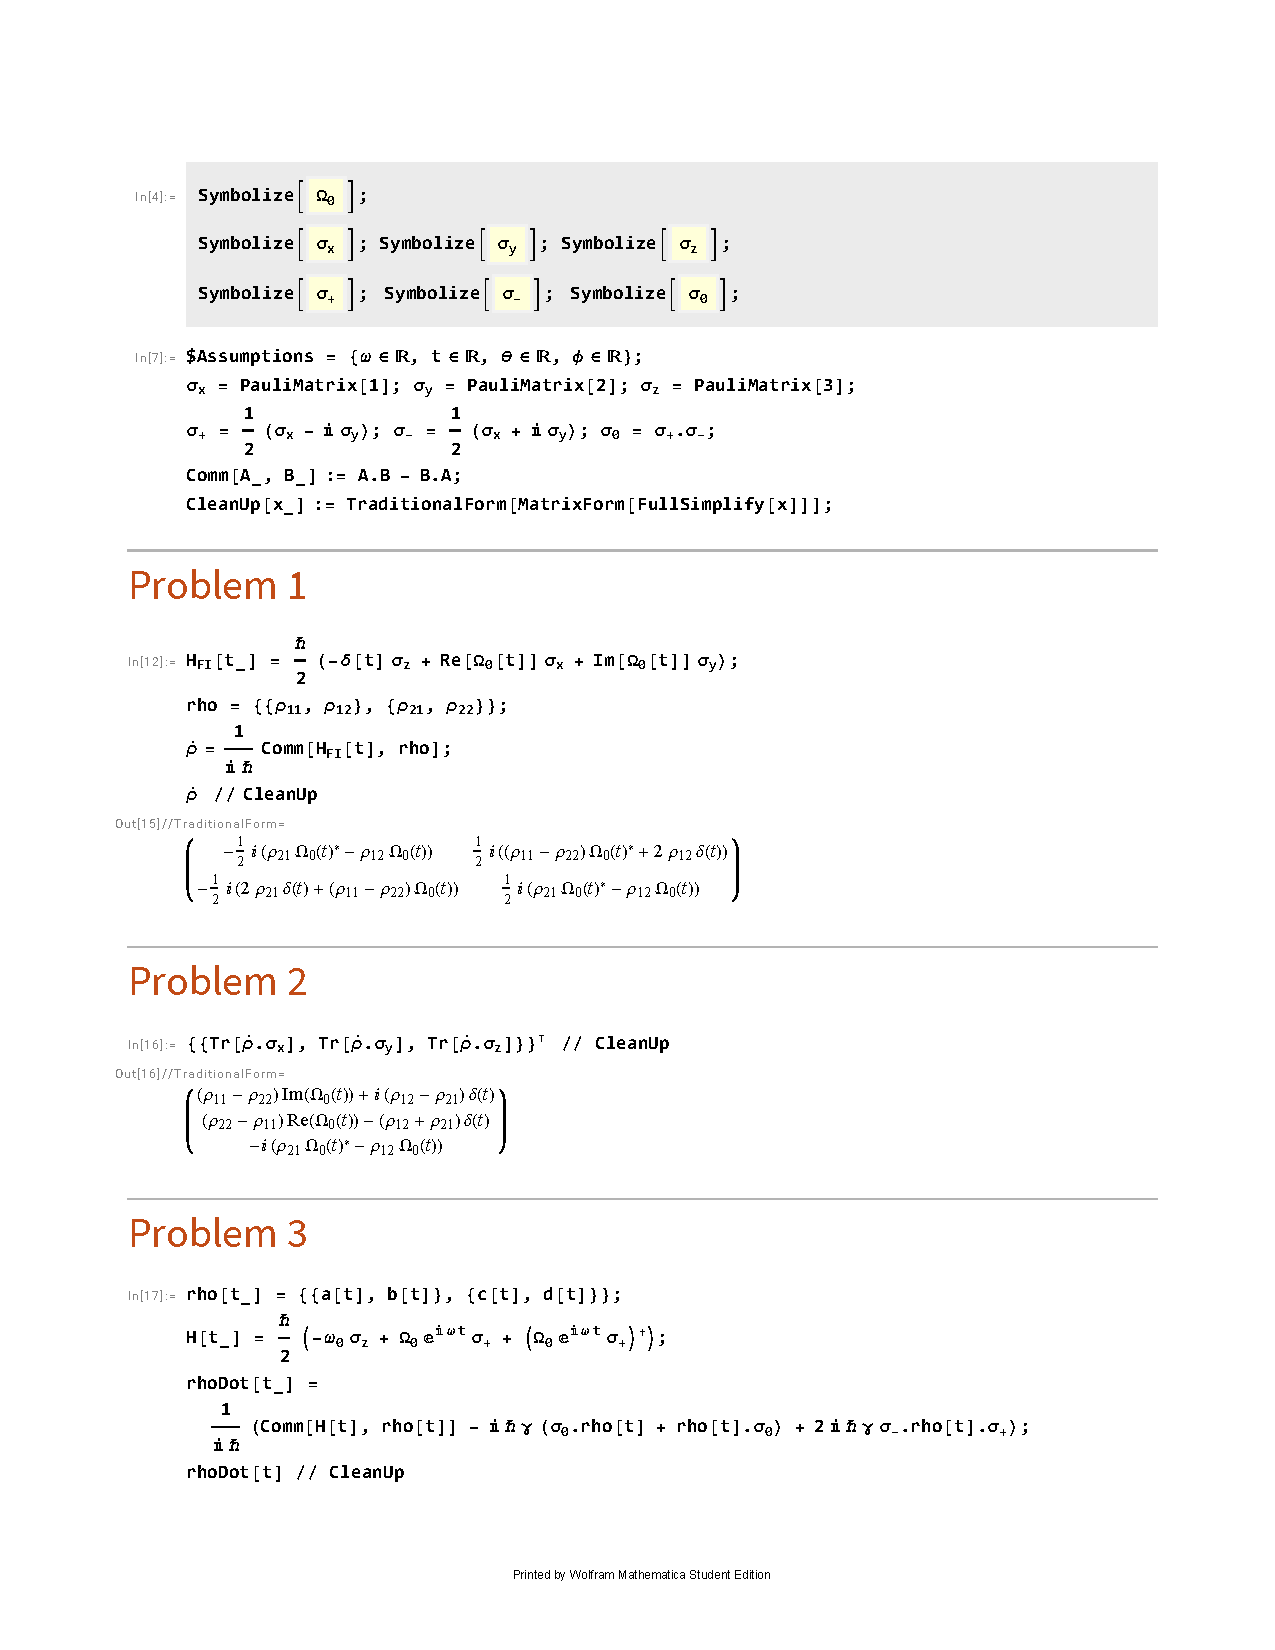
\includepdf[pages=-]{calcs/HW3_mathematica.pdf}
\end{document}